\documentclass[11pt,english,twoside]{article}
\usepackage{katdoc}
\usepackage{graphicx, url,color}
\usepackage{verbatim}

\newcommand{\docClient}{SKA SA and NRF}
\newcommand{\docProject}{CASPER}
\newcommand{\docType}{Data Interface Protocol Definition}

\newcommand{\docId}{SSA4700-0000-001}
\newcommand{\docRevision}{1}
\newcommand{\docClassification}{Open Source, GPL}
\newcommand{\docDate}{2012/10/16}
\newcommand{\docCopyright}{\copyright CASPER 2010}


% Format: \addcontributor{Role}{Name}{Designation}{Affiliation}{Date}
\newcommand{\docApproval}{
    \addcontributor{Submitted by}{R. van Rooyen}{DBE DSP Specialist}{SKA SA}{}
    \addcontributor{Approved by}{M. Welz}{DBE Software}{SKA SA}{}
    \addcontributor{Approved by}{J. Manley}{DBE DSP Specialist}{SKA SA}{}
    \addcontributor{Approved by}{S. Ratcliffe}{SPT Subsystem Manager}{SKA SA}{}
    \addcontributor{Approved by}{A. Parsons}{PI}{PAPER}{}
    \addcontributor{Accepted by}{F. Kapp}{DBE Subsystem Manager}{SKA SA}{}
}

% Format: \addchange{Revision}{Date}{ECN}{Comments}
\newcommand{\docHistory}{
    \addchange{A}{2009/04/17}{N/A}{Misc changes made after meeting between DBE, CSS and DSG teams. Packet header field numbering altered, inclusion of higher resolution fields, etc}
    \addchange{B}{2009/04/30}{N/A}{Added Timestamp scale factor field (47), updated explanation and example meta data packets accordingly}
    \addchange{C}{2009/07/01}{N/A}{Conversion from memo to interface control document}
    \addchange{D}{2009/07/10}{N/A}{Renamed to NRF-FF-ICD-W-402}
    \addchange{E}{2009/07/13}{N/A}{Renamed to NRF-FF-ICD-F-402}
    \addchange{F}{2009/07/20}{N/A}{Made changes requested by Alan, retrospectively changed the version numbers to letters}
    \addchange{G}{2009/07/27}{N/A}{Renamed to K8000-0027V1-002 ICD}
    \addchange{H}{2009/08/05}{N/A}{Changes from internal review}
    \addchange{I}{2009/09/21}{N/A}{Started incorporating changes from OAR of Thomas}
    \addchange{J}{2009/10/27}{N/A}{Renamed to SPADE for public release. Incremented to version 3 of the protocol. Added data descriptors.}
    \addchange{K}{2009/11/09}{N/A}{Renamed to SPEAD. Added unified option and payload descriptor.}
    \addchange{L}{2010/03/21}{N/A}{Misc changes after discussions between J. Manley and A. Parsons.}
    \addchange{M}{2010/06/07}{N/A}{Document revision and renumbering of items.}
    \addchange{N}{2010/08/28}{N/A}{Updating for implementation changes and error correction.}
    \addchange{O}{2010/10/07}{N/A}{First review before document release.}
    \addchange{1}{2012/10/16}{N/A}{First revision release.}
}

% Format: \addprogram{Role}{Package}{Version}{Filename}
\newcommand{\docSoftware}{
    \addprogram{Text processor}{\LaTeX}{3.1415926-1.40.10}
    \addprogram{Editor}{Vim}{7.2.445}
}

% Format: \abbrev{ABBREV}{Definition}
\newcommand{\abbreviations}{
    \abbrev{FF}{Fringe Finder}
    \abbrev{ICD}{Interface Control Document}
    \abbrev{IP}{Internet Protocol}
    \abbrev{KAT}{Karoo Array Telescope}
    \abbrev{KATCP}{KAT Communication Protocol}
    \abbrev{TCP}{Transmission Control Protocol}
}

\newcommand{\applicableDocs}{
  \adddocument{Simon Ratcliffe}{}{https://github.com/ska-sa/PySPEAD}{ 2010}
}

% \newcommand{\referenceDocs}{
%   \adddocument{\label{ref:protocol}Simon Cross, Marc Welz, Jason Manley}{KAT Control Protocol Specification}{\url{http://casper.berkeley.edu/wiki/images/1/11/NRF-KAT7-6.0-IFCE-002-Rev4.pdf}}{October 2012}
% }
\renewcommand{\floatpagefraction}{0.8}

\begin{document}

\title{SPEAD: Streaming Protocol for Exchanging Astronomical Data}
\author{J. Manley, M. Welz, A. Parsons, S. Ratcliffe}
\makekatdocbeginning

\references{spead}

\section{Glossary}
\begin{tabular}{l|p{14cm}}
TCP/IP
&
Transmission Control Protocol (TCP) is a set of rules (protocol) used along with the Internet Protocol (IP) to send data in the form of message
units between computers over the Internet. While IP takes care of delivery of the data, TCP takes care of keeping track of the individual units
of data (called packets) that a message is divided into for efficient routing through the Internet.  \\
& \\
UDP
&
User Datagram Protocol (UDP) uses the IP to transport a data unit (called a datagram) from one computer to another, but UDP makes no guarantee
about data delivery, nor does it provide sequencing of the packets. This means that it is up to the application program that uses UDP to make
sure that the entire message has arrived and is in the correct order.  \\
& \\
Datagram
&
A datagram is a self-contained, independent entity of data carrying sufficient information to be routed from the source to the destination
computer without reliance on earlier exchanges between the source and destination computer and the transporting network. \\
& \\
\emph{Item}
&
A variable transmitted using the SPEAD protocol. \\
& \\
\emph{ItemGroup}
&
A collection of \emph{Items} to be transmitted. \\
& \\
\emph{Heap}
&
An \emph{ItemGroup} packaged for transmission as UDP data packets. \\
& \\
\emph{ItemPointer}
&
Meta data in the packet header containing information on how to unpack the received datagram.
\end{tabular}

\newpage

\section{Scope}

This document describes a data stream format suitable for use by radio astronomy instruments. The data stream is distinct from the KATCP
control protocol described in Reference~\cite{ffdbectl}.

Many instruments output data over Ethernet. These streams are often high speed and unsuitable for TCP/IP links. UDP is often preferred in the
cases where partial data-loss can be accommodated. This document aims to standardise the output format of such UDP streams.

An essential feature of the data stream is that it is self describing.  This self description extends to the content and interpretation of the
optional fields in the packet header, as well as the data payload itself.  The same receive and transmit code may be used for multiple
instruments as the layout of the packets are well defined.

Emphasis is placed on lightweight implementation, suitable for data packetisation by hardware devices or by software processes, while retaining
flexibility for complex, dynamically changing data exchanges. Descoping, by way of fixed packet format, is required for simple receivers.

Metadata and variable descriptors can be injected into the data stream at runtime and recorded or processed along with the primary data stream. It
is also possible to record the raw data stream directly to disk for later parsing. Note: Data flow is unidirectional in a given SPEAD data
stream.

The format of the application-layer packetised stream is described in this document. Lower speed and ad-hoc data products may be transferred
using the TCP-based KATCP control interface~\cite{ffdbectl}.


\section{Protocol Layers}

The data stream format describes the application and presentation layers of the OSI model. Data transmission can take place over any
medium---such as serial data lines, or Ethernet networks---and is generally transmitted via a network interface, or stored on disk.

The preferred interface for network communications consists of the
following layers:
\begin{description}
\item[Application and Presentation]: ~ \\
\hspace{1cm} The data format as described in this document.

\item[Session and Transport]: ~ \\
\hspace{1cm} UDP, noting that the receiving party cannot request retransmission of lost, duplicated or corrupt packets.

\item[Network]: ~ \\
\hspace{1cm} IP (Internet protocol).

\item[Link]: ~ \\
\hspace{1cm} Ethernet (100 GbE, 40 GbE, 10 GbE, GbE, or 100 Mb/s).

\item[Physical]: ~ \\
\hspace{1cm} Any Ethernet medium, such as CFP, QSFP+, SFP+, CX4 or other 10 Gigabit Ethernet cable, Cat6, Cat5e,
etc.
\end{description}


\section{Definition}

The SPEAD protocol is designed to propagate changes in a set of variables from one location to another.  The origin and use of these variables
are application dependent and is, as such, beyond the scope of this document. See KAT-7 data interface document for KAT-7 example
implementation~\cite{speadkat7}.

SPEAD uses the UDP protocol to transmit data packets called datagrams from one computer to another.  Each user-created datagram consists of a
SPEAD header, three or more optional \emph{ItemPointer} fields and a data payload. While SPEAD can cope with lost or missing packets, it has no
mechanism to request resending of missing data.

Different flavours of SPEAD can be created by specifying the number of addressable variables and total variable-space size. The SPEAD flavour is
expressed as SPEAD-\emph{XX-YY} where \emph{XX} is the \emph{ItemPointer} bit length and \emph{YY} is the heap address space; \emph{XX} is
always greater than or equal to \emph{YY}. This format is self-defining and these widths are configurable in the SPEAD header.  Once specified, the
allocated SPEAD sizes (\emph{XX} and \emph{YY}) should remain static for a given implementation.

SPEAD-\emph{64-40} is currently deployed, allowing for data heaps of up to 1T/B (40 bit) and up to $2^{23}$ (8388608) variables (1-bit is
reserved for addressing mode).  The \emph{Heap} size limit (\emph{YY}) does not limit the total size of the SPEAD stream, it merely constrains
the total number of variables \emph{Item}s that can be changed simultaneously.


\section{Data Overview}

Each variable is associated with an \emph{Item}. The \emph{Item} contains:
\begin{itemize}
\item the variable's value, which can be a single-valued data product, multi-dimensional data, or can point to other \emph{Item}s or multiples
of other \emph{Item}s, thereby allowing hierarchical data structures;
\item associated metadata, i.e. the variable name, description, type and shape;
\item a numerical identifier.
\end{itemize}

\begin{figure}[!htb]
\centering
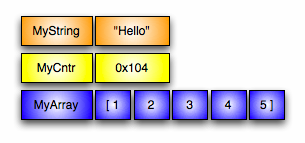
\includegraphics[height=3cm]{images/user_defined_spead_items}
\caption[Example transmit data]{\label{fig:items}\small Consider a grouping of data that we might wish to transmit. It has multiple data
elements, including a string ``MyString'', an integer counter ``MyCntr'', and an array of 32-bit unsigned integers called ``MyArray''.}
\end{figure}

\emph{Item}s are collected into \emph{ItemGroup}s. An \emph{ItemGroup} can be modified by the addition of \emph{Item}s, and by the modification
of an \emph{Item}'s value or its metadata. Once \emph{Item}s in an \emph{ItemGroup} have been modified to a selfconsistent state, the change in
the state of the \emph{ItemGroup} can be encoded as a \emph{Heap}.

The \emph{Heap} is subdivided into a collection of data packets and sent as a stream of UDP datagrams from the transmitter to the receiver.
\emph{ItemPointer}s in the packet header point to an address within an assembled \emph{Heap} of data where the \emph{Item}'s data-products are
stored. This allows for very large data lengths for a given \emph{Item}, which is unrestricted by the packet length. On the receiver, the
\emph{Heap} is reassembled and then unpacked as an \emph{ItemGroup}. All \emph{Item}s can be automatically unpacked and interpreted before
presentation to the user's application.

\emph{ItemPointer}s can be used as either an immediate address or as an absolute address. Immediate addressing refers to using the
\emph{ItemPointer} as a value instead of a pointer. This is more efficient for \emph{Item}s which contain either character or single-valued
items. Absolute addressing refers to using the \emph{ItemPointer} as an address within an assembled \emph{Heap}. This address is a byte offset
within the \emph{Heap} where the \emph{Item}'s data-products are stored.


\section{Data Flow}

A \emph{Heap} consists of a header section, followed by a payload section. The header section is a list of \emph{ItemPointer}s, while the
payload contains \emph{Item}s' values.

The process of encoding changes in \emph{Item}s as a \emph{Heap} proceeds as follows:

\begin{enumerate}

\item For each \emph{Item} whose value has changed, the binary representation of the new value is appended to the \emph{Heap} payload, and an
\emph{ItemPointer} is appended to the \emph{Heap} header.  An \emph{ItemPointer} encodes the \emph{Item}'s numerical identifier, and a byte
offset into the \emph{Heap}'s payload where the \emph{Item}'s value begins.  For the special case where an \emph{Item}'s value fits within the
field allocated for the \emph{ItemPointer} address, the value is not appended to the \emph{Heap}, but is instead placed in the address field,
and a one-bit IMMEDIATE flag in the \emph{ItemPointer} is set to indicate that the value can be accessed directly as illustrated in
Figure~\ref{fig:heap_construct}.
\begin{figure}[!htb]
\centering
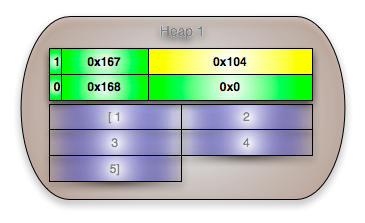
\includegraphics[height=4cm]{images/spead_heap_construct}
\caption[Example \emph{Heap} construct]{\label{fig:heap_construct}\small An example \emph{Heap} of \emph{Item}s to transmit: user-defined
\emph{Item} with identifier 0x167 has an integer value of 0x104 and is included directly into the header (with the IMMEDIATE flag set to 1),
while user-defined \emph{Item} 0x168's value can be found at \emph{Heap} offset 0x0.}
\end{figure}


\item An \emph{ItemDescriptor} is generated for each new \emph{Item} that has been added to the \emph{ItemGroup}, that is, the first time
this variable is created. An \emph{ItemDescriptor} is also created when a specific \emph{Item}'s structure has changed.  The value of an
\emph{ItemDescriptor} is itself a \emph{SpeadStream} that may contain such \emph{Item}s as NAME, DESCRIPTION, TYPE, SHAPE, and ID.  The binary
representation of this \emph{SpeadStream} is appended to the \emph{Heap} payload, and a special \emph{ItemPointer} is added to the header of the
\emph{Heap} that has its numerical identifier set to DESCRIPTOR\_ID, and points to the start of the \emph{ItemDescriptor}'s value in the
\emph{Heap} payload. The reader is referred to the section on \emph{ItemDescriptor}s for more detail.

\item This \emph{Heap} is now converted into a series of SPEAD packets.  Each packet consists of a SPEAD header, a number of
\emph{ItemPointer}s, and a payload.  With the exception of some \emph{ItemPointer}s added to aid in packet decoding and reassembly,
all \emph{ItemPointer}s are drawn from the \emph{Heap} header.  Each packet payload contains a portion of the \emph{Heap} payload.  Taken
together, the generated series of packets will contain the entirety of the \emph{Heap}'s header and payload, along with a small number of
IMMEDIATE \emph{ItemPointer}s that allow each packet to be associated with reconstructing a single \emph{Heap} on the receive side.

\item After packets pass through a physical transport layer -- such as a network interface, POSIX pipe, file -- a receiver sorts incoming
packets by associated \emph{Heap} and begins the process of reconstructing the \emph{Heap}.  Packet headers are concatenated into a \emph{Heap}
header, and packet payloads are concatenated in the correct order to reconstruct the \emph{Heap} payload. Missing packets are flagged.

\item Next, each \emph{ItemPointer} in the \emph{Heap} header is processed, associating a numerical identifier with a the binary value.  For
DIRECT-addressed \emph{ItemPointer}s, this involves seeking within the \emph{Heap} payload to the specified address offset and extracting data
from that point to the start of the next \emph{ItemPointer}.  For IMMEDIATE \emph{ItemPointer}s, the binary value is extracted directly from the
address field.

\item Finally, the receiver's \emph{ItemGroup} associates each numerical identifier and binary value pair with an \emph{Item} having the same
identifier.  All \emph{ItemPointer}s are processed, creating new \emph{Item}s when appropriate.  Each binary value is then decoded to an actual
value by using the structure information provided by the associated \emph{ItemDescriptor}.

\end{enumerate}


\section{Packet Data Representation}

Data is always transmitted and stored most significant bit first, that is, Internet Protocol standard byte ordering.  Because this same ordering
is used for on-disk storage, data can be streamed directly between the network and storage.

At a minimum, a SPEAD packet must contain the following, as illustrated in Figure~\ref{fig:packet_construct}:
\begin{itemize}
\item A SPEAD header
\item Three \emph{ItemPointer}s, in no particular order, describing:
  \begin{itemize}
    \item the packet payload length to locate packet boundaries for on-disk storage,
    \item the offset of this packet's contents within the \emph{Heap},
    \item and a counter, timestamp, or other unique number indicating the \emph{Heap} to which it belongs.
  \end{itemize}
\end{itemize}

\begin{figure}[!htb]
\centering
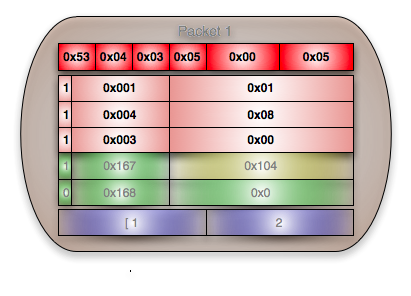
\includegraphics[height=5cm]{images/spead_packet_construct}
\caption[\emph{Heap} packet example]{\label{fig:packet_construct}\small Example SPEAD-64-40 packet containing 5 \emph{Item}s. This packet
belongs to \emph{Heap} 1 and has a payload that is 8 bytes long which starts at \emph{Heap} offset 0x00 i.e. this is the first packet of the
\emph{Heap}.}
\end{figure}


\subsection{SPEAD header}

The SPEAD header is always 8 octets (64 bits) long. All packets have a header of the following form:

\begin{tabular}{|c|c|c|c|c|c|}
\hline
\emph{MSb} &&&&& \emph{LSb} \\
\hline
Magic \# (8b) & Version (8b) & ItemPointerWidth (8b) & HeapAddrWidth (8b) & Reserved (16b) & \# Items (16b)\\
\hline
\end{tabular}

\begin{description}

\item[MagicNumber]:
This is a constant value. All packets will start with the following 8 bit pattern: \emph{(msb) 0101 0011 (lsb)} which has a numerical value of
0x53 and represents an ASCII \emph{S}.  This allows basic identification of the packet as a SPEAD packet.

\item[Version]:
This field identifies the version of the packet format. Designed in case future packet structures differ. The version described here is 4.

\item[ItemPointerWidth and HeapAddressWidth]:
These fields describe the number of bytes of each \emph{Heap} address (\emph{HeapAddressesWidth}) and the total size of an
\emph{ItemIdentifier}, the \emph{ItemIdentifierWidth}. The sum of the two numbers indicate the size of an \emph{ItemPointer}.

Initial implementations of SPEAD (SPEAD-64-40) have 64 bit \emph{ItemPointer} fields, of which 40 bits address the data in a \emph{Heap}, one
bit chooses the addressing mode and the remaining 23 bits represent a numeric \emph{ItemIdentifier}.  HeapAddressWidth is thus set to $40
\mbox{bits} /8 \mbox{bits} =5$ bytes and ItemPointerWidth set to $24 \mbox{bits} /8 \mbox{bits} =3$ bytes, which includes the ItemPointerWidth
which is the one bit, the MSB, always used for Addressing mode. This configuration defines the flavour of SPEAD and is referenced as
SPEAD-64-40.  These numbers need to remain static for a given configuration or implementation once the stream has started.

\item[Reserved]:
This field should be ignored. The space is reserved for future allocation.

\item[NumberOfItems]:
The value stored in this field indicates the number of \emph{ItemPointer}s contained in this packet. \emph{ItemPointer}s follow immediately
after the SPEAD header. The packet payload follows directly after these \emph{ItemPointer} fields. This field allows the offset of the payload
to be determined.

\end{description}


\subsection{\emph{ItemPointers}: optional fields}

\emph{Item}s are used to transfer variables. Each packet can contain a variable number of data fields, called \emph{ItemPointer}s, which follow
directly after the SPEAD header. Each \emph{ItemPointer} consists of some bits of \emph{ItemIdentifier} and some bits of \emph{ItemAddress}, a
pointer to the location of the data in the \emph{Heap}, in direct address mode, or the data itself, in immediate address mode.

\emph{ItemPointer}s can have a user-defined length, which defines the flavour of the SPEAD protocol employed. See above description for more
information on sizing these fields.

The number of \emph{ItemPointer}s in a packet is defined by the \emph{NumberOfItems} field in the SPEAD header, and should be 3 or more; a
minimum of 3 are required by SPEAD.

\begin{description}

\item[ItemAddressMode]: An \emph{ItemPointer}'s lower bits, the \emph{ItemAddress} field, normally store the \emph{Heap} address where that
\emph{Item}'s data can be found. This is called absolute addressing mode.

Alternatively, the \emph{ItemAddress} field can store the \emph{Item}'s value. This is called immediate addressing mode.

Using immediate addressing allows for data widths of up to \emph{HeapAddressWidth} bytes to be accommodated without incurring the additional
overhead of a pointer. Whereas using a pointer in direct addressing mode allows for lengths of data longer than \emph{HeapAddressWidth} bytes.

The addressing mode, and hence the interpretation of the \emph{ItemAddress} field, is determined by the first bit in the \emph{ItemPointer}. If
this bit is clear, the \emph{ItemAddress} field is interpreted as an index into the payload of the \emph{Heap} and is a direct address.  If this
bit is set, the associated address is interpreted to immediately contain the value of the \emph{Item} and is an immediate address.

\item[ItemIdentifier]: This field (23 bits for SPEAD-64-40) contains a numerical identifier that associates this \emph{ItemPointer} with a
corresponding \emph{Item} whose value is being updated.

\item[ItemAddress]: The address (40 bits for SPEAD-64-40) can contain either a direct address into the \emph{Heap} where the value for this
\emph{Item} is located, or it can contain the \emph{Item}'s value.  The interpretation of this field depends on how the \emph{ItemAddressMode}
field is set.

\end{description}

Example of an \emph{ItemPointer} in SPEAD-64-40:

\begin{tabular}{|c|c|c|}
\hline
\emph{MSb} && \emph{LSb} \\
\hline
ItemAddressMode (1b) & ItemIdentifier (23b) & ItemAddress (40b)\\
\hline
\end{tabular}

If a packet is received that contains an unknown \emph{Item}, it might be recorded and ignored or otherwise the receiver might request a
metadata reissue to explain the content (see item 0x0005, the ITEM\_DESCRIPTOR \emph{Item}). In any case, the reception of unknown \emph{Item}s
should not be considered illegal and should be handled cleanly by a receiver.

Generally the \emph{Item}s will be self defining and thus do not need strict identification in this document. However, it is necessary to define
a few \emph{Item}s which will be used for stream configuration and control.

The following table defines these standardised \emph{ItemIdentifier}s and their meaning. Note that some of these require certain address modes.

\begin{tabular}{|r|l|l|l|}
\hline
\emph{Dec} & \emph{Hex} & \emph{Description} & \emph{Addr mode} \\
\hline
 0 & 0x0000 & NULL - Ignore            & Ignored   \\
 1 & 0x0001 & Heap counter             & Immediate \\
 2 & 0x0002 & Heap size                & Immediate \\
 3 & 0x0003 & Heap offset              & Immediate \\
 4 & 0x0004 & Packet payload length    & Immediate \\
 5 & 0x0005 & Item descriptor          & Absolute  \\
 6 & 0x0006 & Stream control           & Immediate \\
16 & 0x0010 & Item descriptor: name    & Not specified \\
17 & 0x0011 & Item descriptor: description & Not specified \\
18 & 0x0012 & Item descriptor: shape   & Not specified \\
19 & 0x0013 & Item descriptor: type    & Not specified \\
20 & 0x0014 & Item descriptor: ID      & Immediate \\
21 & 0x0015 & Item descriptor: dtype   & Absolute \\
\hline
\end{tabular}

The remaining \emph{ItemIdentifier} address space is available for user specification. It is recommended that users' applications start at
\emph{Item} \#1024.

Herewith follows an explanation for these standard \emph{Item}s:


\subsubsection{NULL}

This \emph{Item} is used for optional data padding and can be ignored by the receiver.


\subsubsection{Heap counter}

Required field.

Normally just a counter that increments with each \emph{Heap} update. This number does not need to be continuous or even monotonic, but must be
unique. It is used to identify the \emph{Heap} to which a packet belongs.
\begin{description}
\setlength{\itemindent}{0.5cm}
\setlength{\itemsep}{0ex plus0.2ex}
\item[Numerical Identifier]: 0x0001
\item[Name]: heap\_counter
\item[Description]: Identify to which \emph{Heap} a packet belongs.
\item[Type]: unsigned integer, immediate addressing.
\item[Shape]: 1
\end{description}


\subsubsection{Heap size}

Optional \emph{Item}.

It is highly recommended that this \emph{Item} be issued for each \emph{Heap} to allow receivers to detect when a \emph{Heap} is complete (as opposed
to waiting for a timeout or buffer overflow).
\begin{description}
\setlength{\itemindent}{0.5cm}
\setlength{\itemsep}{0ex plus0.2ex}
\item[Numerical Identifier]: 0x0002
\item[Name]: heap\_size
\item[Description]: Specify the total size of the \emph{Heap}, up-front, in bytes. Allows processing right after reception of last packet of the
\emph{Heap}.
\item[Type]: unsigned integer, immediate addressing.
\item[Shape]: 1
\end{description}


\subsubsection{Heap offset}

Required field.

The position relative to the start of this \emph{Heap}, at which the payload of the current packet starts. It is used for re-assembling a
\emph{Heap} that was split across multiple packets. It is reset back to zero for the following \emph{Heap}.

For example, in a correlator, this field would typically measure the byte offset from the start of an integration, as each integration would
constitute another \emph{Heap}.

\begin{description}
\setlength{\itemindent}{0.5cm}
\setlength{\itemsep}{0ex plus0.2ex}
\item[Numerical Identifier]: 0x0003
\item[Name]: heap\_offset
\item[Description]: The position in bytes relative to the start of this \emph{Heap} at which the payload of the current packet starts.
\item[Type]: unsigned integer, immediate addressing.
\item[Shape]: 1
\end{description}


\subsubsection{Packet payload length}

Required field.

This is the size in bytes of the packet payload length, excluding the header and item fields.

\begin{description}
\setlength{\itemindent}{0.5cm}
\setlength{\itemsep}{0ex plus0.2ex}
\item[Numerical Identifier]: 0x0004
\item[Name]: pkt\_len
\item[Description]: The length in bytes of this packet's payload.
\item[Type]: unsigned integer, immediate addressing.
\item[Shape]: 1
\end{description}


\subsubsection{Stream control}

Optional \emph{Item}.

\begin{description}
\setlength{\itemindent}{0.5cm}
\setlength{\itemsep}{0ex plus0.2ex}
\item[Numerical Identifier]: 0x0006
\item[Name]: stream\_ctrl
\item[Description]: Indicates the status of the SPEAD stream.
\item[Type]: unsigned integer, immediate addressing.
\item[Shape]: 1
\end{description}

The STREAM\_CONTROL \emph{Item} can indicate the one of the following status for a SPEAD stream:

\begin{description}
\item[0]:   Stream start
\item[1]:   \emph{ItemDescriptor} reissue (see section below on \emph{ItemDescriptor}s)
\item[2]:   Stream stop
\item[3]:   \emph{ItemDescriptor} update (\emph{Item} has changed dimensions)
\item[>=4]: Reserved for future use. Ignore.
\end{description}


\subsection{\emph{ItemDescriptors}}

\emph{ItemDescriptor}s are used to provide receiving clients with the metadata required to decode, interpret and unpack \emph{Heap}s to form
\emph{ItemGroup}s as part of a particular SPEAD stream. In general, these packets will be sent at the start of a session before data packet
transmissions begin.

\emph{ItemDescriptor} updates can be issued at any time, including during a data stream. Such re-issuances are encouraged, so that if a receiver
were to fail or lose state, it can recover and continue processing incoming data. Such packets may or may not contain a STREAM\_CONTROL
\emph{Item} with the value of 1 (\emph{ItemDescriptor} reissue).

Updates to \emph{Item}s that are captured together with data, i.e. as part of the same \emph{Heap}, are applied immediately to that captured
\emph{Heap} prior to unpacking or data interpretation. This allows the user to change object dimensions on-the-fly. Such data may or may not be
accompanied by a STREAM\_CONTROL \emph{Item} with the value of 3 (\emph{ItemDescriptor} update).

\emph{ItemDescriptor}s are themselves complete SPEAD packets, including the SPEAD header (see Appendix for example usage). Each \emph{ItemDescriptor} should contain at least the
following \emph{Item}s:

\begin{description}
\item[ItemDescriptorID]: The numerical code used to identify the \emph{Item} that we are describing. It has a bitwidth of $ItemPointerWidth -
HeapAddressWidth - 1$.
\item[ItemDescriptorName]: A short string identifying the variable contained in this \emph{Item}.
\item[ItemDescriptorDescription]: A human-readable string explaining the variable's use and packing scheme.
\item[ItemDescriptorType]: A binary-packed string representing the data type (signed or unsigned integer, float, string, boolean etc) and number
of bits per value.
\item[ItemDescriptorShape]: A binary-packed string representing the size along each dimension.
\item[ItemDescriptorDType]: An optional string specifying the shape and type of this item using numpy dtype string syntax.
\end{description}


\subsubsection{ItemDescriptorID}

The value of this \emph{ItemDescriptor} \emph{Item} is the identifier of the \emph{Item} that we are trying to describe in this
\emph{ItemDescriptor}.

\begin{description}
\setlength{\itemindent}{0.5cm}
\setlength{\itemsep}{0ex plus0.2ex}
\item[Numerical Identifier]: 0x0014
\item[Name]: descriptor\_id
\item[Description]: The numerical code used to identify the \emph{Item} described by this \emph{ItemDescriptor}.
\item[Type]: unsigned integer, immediate addressing.
\item[Shape]: 1
\end{description}

\subsubsection{ItemDescriptorName}

Payload names are intended to be parsed and presented in the receiver namespace and thus should not include whitespace (including [LF], [FF]
etc).

SPEAD does not mandate a maximum length for this field. It will be unpacked as the variable name by the receiver, so this should not be a
verbose field. Use \emph{ItemDescriptorDescription} for detailed explanations.

\begin{description}
\setlength{\itemindent}{0.5cm}
\setlength{\itemsep}{0ex plus0.2ex}
\item[Numerical Identifier]: 0x0010
\item[Name]: descriptor\_name
\item[Description]: The variable name used to identify the \emph{Item} described by this \emph{ItemDescriptor}.
\item[Type]: string
\item[Shape]: \emph{variable length, single dimension}
\end{description}


\subsubsection{ItemDescriptorDescription}

\begin{description}
\setlength{\itemindent}{0.5cm}
\setlength{\itemsep}{0ex plus0.2ex}
\item[Numerical Identifier]: 0x0011
\item[Name]: descriptor\_description
\item[Description]: The human-readable description of the \emph{Item} described by this \emph{ItemDescriptor}.
\item[Type]: string
\item[Shape]: \emph{variable length, single dimension}
\end{description}


\subsubsection{ItemDescriptorType}

\begin{description}
\setlength{\itemindent}{0.5cm}
\setlength{\itemsep}{0ex plus0.2ex}
\item[Numerical Identifier]: 0x0013
\item[Name]: descriptor\_type
\item[Description]: Machine-parsable string detailing this \emph{Item}'s binary packing.
\item[Type]: string
\item[Shape]: \emph{variable length, single dimension}
\end{description}

This \emph{Item} contains an unpack string telling the parser how to unpack the payload, and follows a C style printf convention, with the
addition of referenced data types. The \emph{ItemType}'s string payload can contain one or more unpack directives, with each directive referring
to a consecutive data type in the payload. Each directive has the following form: \emph{unpack\_type[bit\_length | ItemIdentifier]}.

\begin{tabular}{|r|l|l|}
\hline
\emph{ASCII} & \emph{Hex} & \emph{Representation} \\
\hline
0 & 0x0030 & interpret remaining XX bits as an \emph{ItemIdentifier} \\
i & 0x0069 & signed integer \\
u & 0x0075 & unsigned integer \\
f & 0x0066 & IEEE float \\
c & 0x0063 & ASCII character \\
b & 0x0062 & boolean \\
\hline
\end{tabular}

The unpack character `0' allows the unpack string to reference another \emph{Item}, thus allowing hierarchical constructs. Where the
\emph{bit\_length} (or \emph{ItemIdentifier}) field has the same size as your SPEAD flavour's ItemIdentifierWidth.


\subsubsection{ItemDescriptorShape}

\begin{description}
\setlength{\itemindent}{0.5cm}
\setlength{\itemsep}{0ex plus0.2ex}
\item[Numerical Identifier]: 0x0012
\item[Name]: descriptor\_shape
\item[Description]: Binary packed vector explaining the shape of this \emph{Item}, in terms of the number of \emph{ItemTypeItems} per
dimension.
\item[Type]: binary packed vector
\item[Shape]: \emph{variable length binary field with one dimension}
\end{description}

The \emph{ItemShape} string allows multiple data constructs of the type specified in the \emph{ItemType} unpack string to be placed contiguously
in the data stream. These values are binary packed integer values. It has the following form:
\begin{verbatim}
count_axis1[,count_axis2[,count_axis3 [...]]]
\end{verbatim}

where each count\_axis field is \emph{HeapAddrWidth}+1 bytes long. The LSb of the first byte of this field indicates if the value is given
immediately or otherwise references another item, i.e. it is possible to have variable-length arrays. This size allows indexing of a 1 bit vector
along the entire heap.

\subsubsection{ItemDescriptorDType}

\begin{description}
\setlength{\itemindent}{0.5cm}
\setlength{\itemsep}{0ex plus0.2ex}
\item[Numerical Identifier]: 0x0015
\item[Name]: descriptor\_dtype
\item[Description]: String representation of numpy dtype.
\item[Type]: string
\item[Shape]: \emph{variable length, single dimension}
\end{description}

The optional descriptor dtype allows specification of the type and shape of an \emph{Item} using a numpy style dtype string. If this string is
present the specified shape and type fields, if any, are ignored and populated from the decoded numpy dtype.

The current reference implementation makes use of this dtype specifier to unpack items directly to numpy arrays, realising a significant
speedup. Thus, the advantage of this parameter may depend on the specific receiver implementation in use.


\subsubsection{\label{sec:ex_descript}Example \emph{ItemDescriptor}}

For example, if the user wished to pack a 100x100 pixel RGB-24 image consisting of 8 bit numbers, you might use the following
\emph{ItemDescriptor} (as illustrated in Figure~\ref{fig:example}).

\begin{description}
\setlength{\itemindent}{0.5cm}
\setlength{\itemsep}{0ex plus0.2ex}
\item[descriptor\_identifier]: 0x5555 \\
Assign numerical identification code as an unsigned integer with immediate addressing.
\item[descriptor\_name]: "my\_picture" \\
Short string of length 10 characters interpreted as variable name.
\item[descriptor\_description]: "A 100x100 pixel RGB-24 image consisting of structs of unsigned 8b red, 8b green and 8b blue data. Data is packed
in rows (i.e. you get 100 pixels from row-1, followed by 100 pixels from row-2 etc)." \\
A verbose, human readable string of length 195 characters.
\item[descriptor\_type]: u8u8u8 \\
\emph{ItemDescriptorType} represents the data type (1 byte) and number of bits per component (with bitwidth defined by the ItemIdentifierWidth of
24 bits). Thus, the number of bytes required to represent the type description: 3(1+24/8) = 12 bytes.
\item[descriptor\_shape]: 100,100 \\
\emph{ItemDescriptorShape} is read as a sequence of unsigned integers representing the variable size along each dimension. The number of bytes
required to represent the shape description is defined by the HeapAddressWidth (40 bits) + 1 byte: 2(1+40/8) = 12 bytes. For this example the
LSb of the first byte of each component is zero (0), indicating that dimensions value follows immediately. (If the LSb of the first byte is one
(1), it indicates that a pointer to another \emph{Item} follows).
\end{description}

The type and shape fields shown above could be replaced by a numpy dtype string:

{\bf descriptor\_dtype}: "`descr':`u1', `fortran\_order':False, `shape':(100,100,.3),"

\begin{figure}[!htb]
\centering
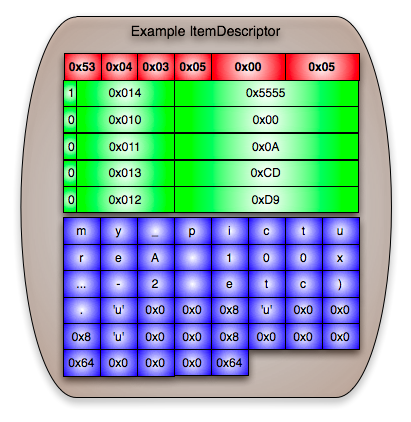
\includegraphics[height=5cm]{images/example_spead_itemdescriptor}
\caption[Example \emph{ItemDescriptor} construct]{\label{fig:example}\small Example \emph{ItemDescriptor} constructed from metadata provided
above.}
\end{figure}


\section{Extra features}


\subsection{HEAP processing}

Normally, the system waits for the first packet from the next \emph{Heap} to arrive before beginning processing of the currently received
\emph{Heap}. This feature is useful when heap sizes need to be flexible. This is typical when the receiver does not know when it has received
all the data for a \emph{Heap}.

However, if the receiver knows the size of the heap beforehand, it can start unpacking as soon as all data has arrived. This allows the protocol
to deal with systems which needs to transmit a response to an incoming data stream before receiving the next piece of data (see \emph{Item} ID
0x0002).

It is also possible to have multiple \emph{Heap}s open at the same time. This is due to network reordering of UDP packets, the system can have
packets from multiple \emph{Heap}s being received at the same time. In this case you do not want to start processing the previous \emph{Heap}
until you are satisfied that all packets have arrived.

Buffer "windows" allow temporary storage of incoming packets associated with up to (N-1) \emph{Heap}s. The system will wait for the first
packet of the N$^{th}$ \emph{Heap} to begin processing of the the \emph{Heap} with the lowest heap counter (see \emph{Item} ID 0x0001).

In general, it is highly recommended that the user transmits the heap size (\emph{Item} ID 0x0002) wherever possible.


\appendix

\newpage
\clearpage
\section{Example Packet Exchange}

To illustrate the process of encoding and assigning new \emph{Item}s we consider an example where we want to transmit the 3 variables described
in Figure~\ref{fig:items} found in the Data Overview Section. These variables are a string, MyString, an integer counter, MyCntr, and an array
of 32-bit unsigned integers, MyArray.
\begin{enumerate}
\item For each new variable an \emph{ItemDescriptor} is generated. This is necessary for the receiving system to know how to interpret and
unpack the data. These packets must be sent before data transmission begins.

\item \emph{ItemDescriptor}s are issued once, at the start of the stream and then only need to be re-sent if parameter shapes change. Full
\emph{ItemDescriptor} packets can also be regenerated upon request through out-of-band signalling, allowing a receiver to process a stream which
had been started earlier.

When a data stream terminates, a further packet may be sent. This may contain a stream control \emph{Item} to indicate that the transmission has
completed.

\item During transmission of the data stream, packets should contain only the changed \emph{Item} fields, in order to maximise the utilisation
of the link. The receiver keeps previous state of \emph{Item}s. Thus, it is only when the value of an \emph{Item} changes that it need to be
retransmitted.

\item Received \emph{ItemPointer}s are added to the associated \emph{Heap}. The immediate-addressed \emph{Item} with identifier 0x167's (MyCntr)
value is available immediately. \emph{Item} 0x168 (MyArray) must wait for the \emph{Heap} unpack before processing. Packet 1's payload is
inserted into \emph{Heap} 1 at offset 0x0. Packet 2 is still pending and the data from \emph{Item} 0x168 is only partially available.
\end{enumerate}

\begin{figure}[!htb]
\centering
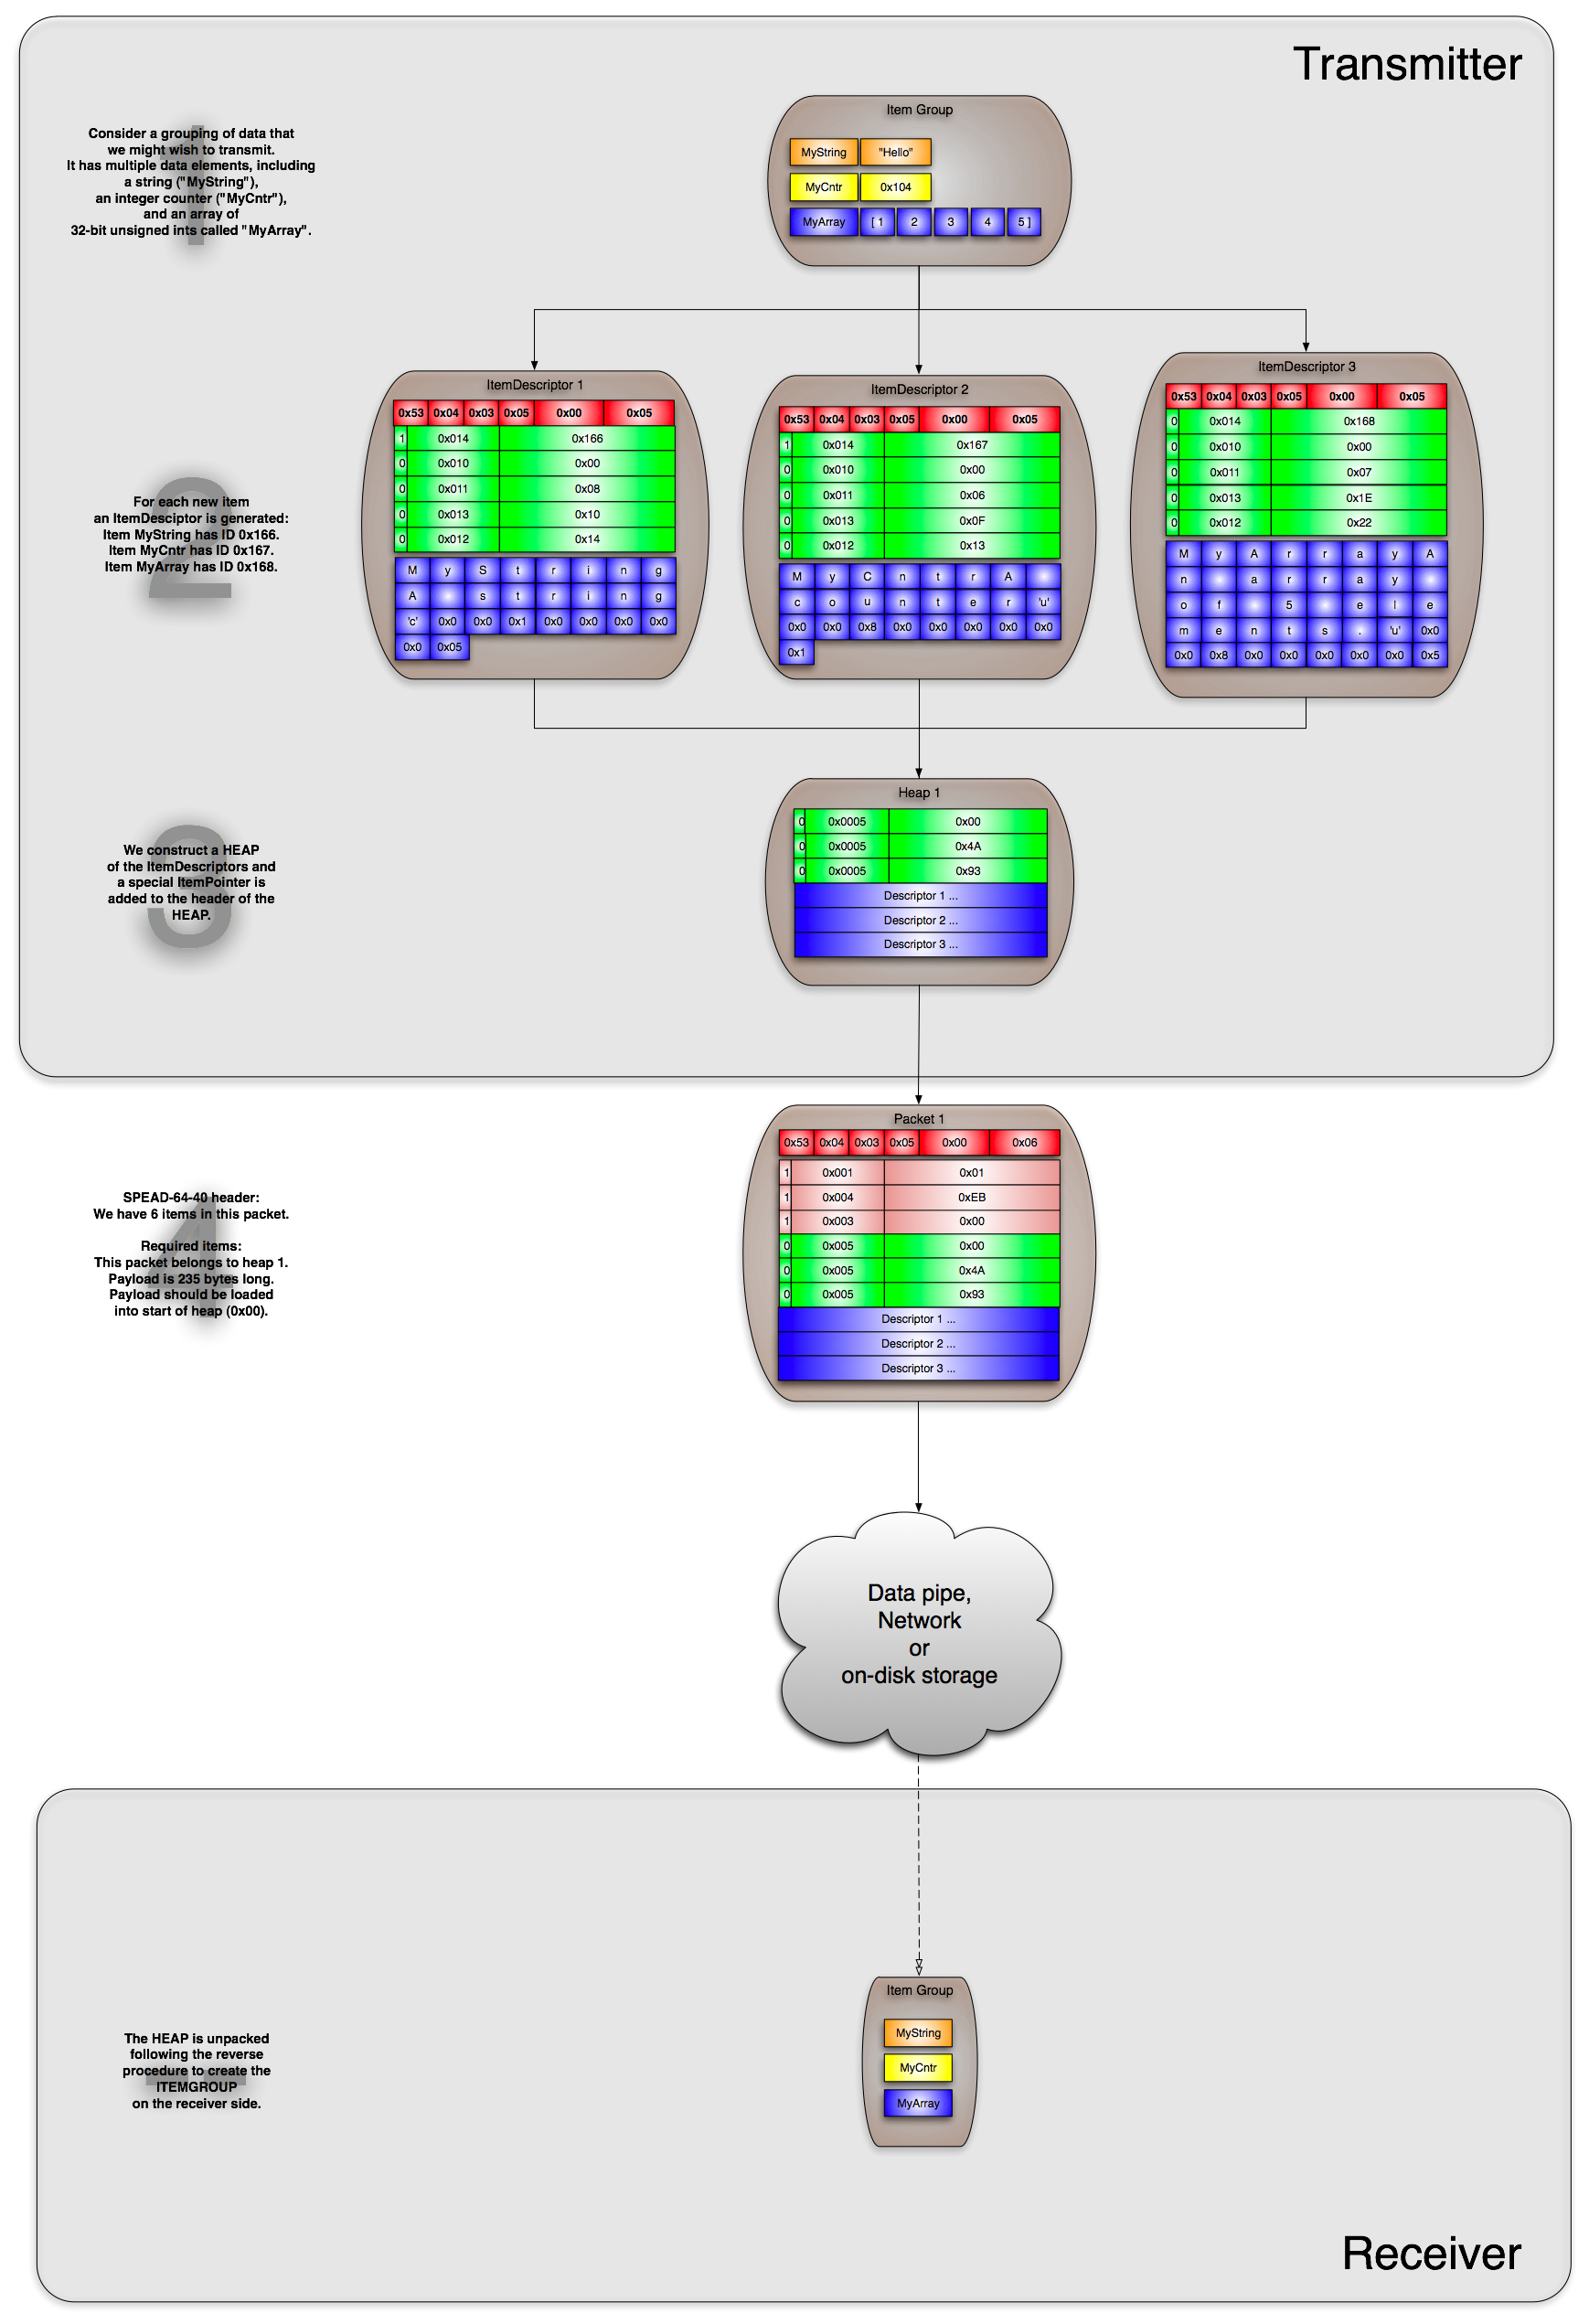
\includegraphics[width=15cm]{images/Spead_itemdescriptor_transmit2}
\caption[Example \emph{ItemDescriptor} exchange]{\label{fig:desc_transmit}\small Creating \emph{ItemDescriptor}s to define 3 variables for
transmission using SPEAD-64-40.}
\end{figure}

\begin{figure}[htbp]
   \centering
   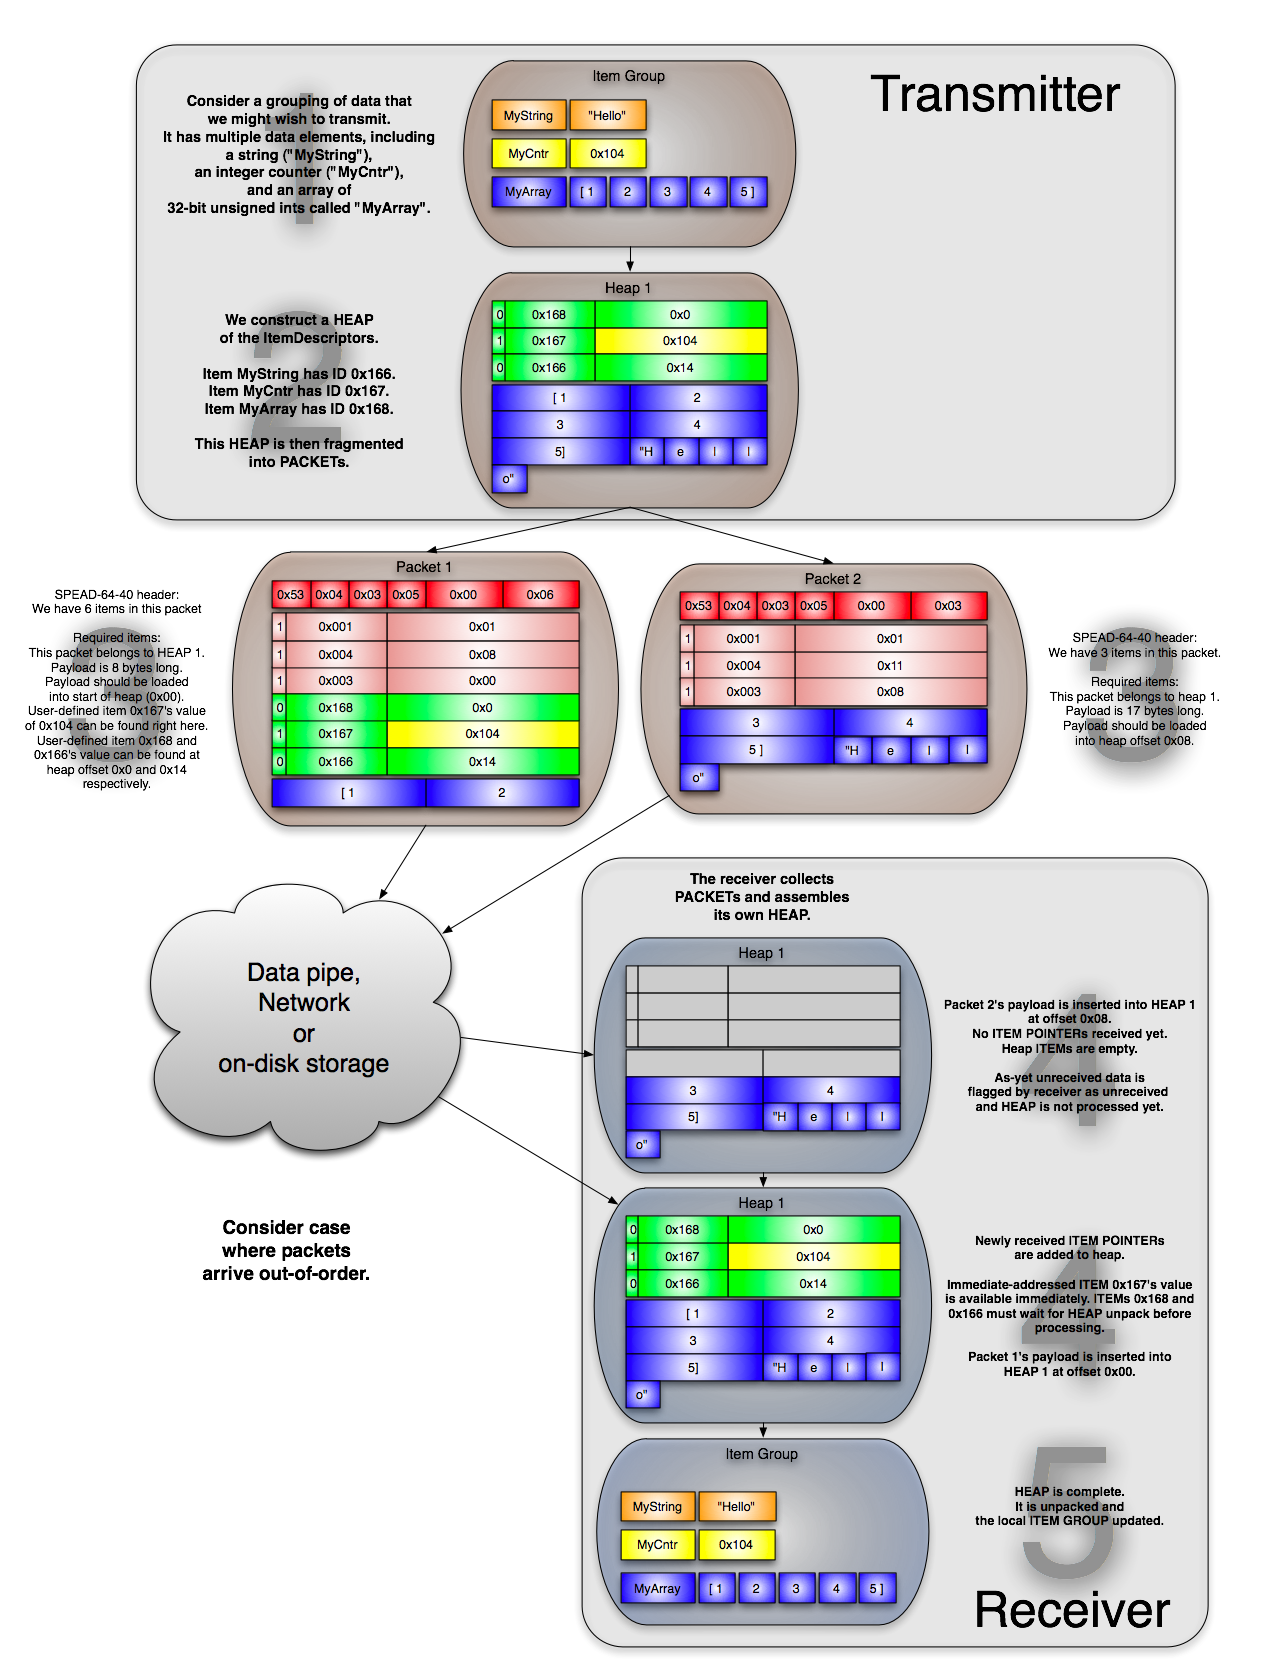
\includegraphics[width=15cm]{images/Spead_itemdescriptor_data2}
   \caption[Example data exchange]{\small Once an \emph{Item} has been described, data packet transmission can begin. In Step 3 of this example
we use ridiculously small packets to demonstrate fragmentation.}
   \label{fig:example_item_desc_exchange}
\end{figure}

\end{document}

